\chapter{TRASH IN CULTURE AND THEORY}




% Epigraph
\begin{singlespace}
% FROM Uncle Fernando’s Garbage Triptych, http://alphabet-city.org/issues/trash/articles/uncle-fernando-s-garbage-triptych, http://priscilauppal.ca/books/alphabet-city/
\epigraph{Anger is nothing compared to garbage:\\Garbage eats anger for breakfast.\\It eats all of us in the end.}{\hfill---Priscilla Uppal, \quotes{Uncle Fernando’s Garbage Triptych}}
\end{singlespace}




%
%
In this chapter trash and the practice of transforming it is examined in theoretical and conceptual aspect. Referred to the ideas and work of philosophers and anthropologists to establish a better understanding of trash beyond common perception and dictionary meaning of it. 

Firstly, I focused on the disposable items that are designed to be ended up in waste bin after a single use. Their usage and place are examined in the society and how other artists used and transformed them is analyzed. Further, disposable items are one of the key material used in the thesis project. Therefore, they need to be discussed in detail.

Secondly, I looked through the Zizek's comments on ecological perspectives that dominate the approaches on rubbish.

Lastly, through "Rubbish Theory" transformation of trash and its various status as an object category that is not static is examined.  





%
%
\section{Throw away culture}





% TODO ref Life Magazine, 1955, "Throwaway Living", p43
%\summary{Throwaway Society} 
%\cite[43]{life1955throwaway} 
Life magazize published an article titled \quotes{Throwaway Living} and proclaimed the arrival of the \quotes{throwaway society} in 1955. It is described as behavioral consumption pattern of society based on throwing away objects after use. The article addresses the question of 
% https://nerc.org/news-and-updates/blog/nerc-blog/2014/01/14/throw-away-society
\quotes{why [to] spend valuable time washing and reusing household objects like plates and silverware when they can be inexpensively made of plastic and disposed of after use?} \citep{tully2014throw} In fact, the term  \quotes{throwaway society} is a critic of it by mentioning its wastefulness and has a slightly negative connotation. 

According to findings of archaeologist Daniel Ingersoll the age of the throwaway world began not in the twentieth century but during the nineteenth \citep[41]{rathje1992rubbish} On the other hand, scholars have criticized the notion of \quotes{throwaway society} as being insufficient and over generalization of consumer behavior \citep{gregson2007identity}. According to the result of their qualitative research on consumers over two-year people are not as wasteful as claimed when considering household possessions such as television, furniture and toys. However, their research did not include disposable packaging and bottles. Therefore, the act of throwing away can be narrowed down to the specific goods.

In this thesis dealt specifically with industrially produced consumer discards and their subsequent transformation. This thesis is necessarily situated at a particular time, place, and sensibility: the consumer culture of the late twentieth century. In its most basic form, consumer culture can be explained, as "the activities and ethics of a society are determined by patterns of consumption" rather than production 
%\todo{ref. Mamiya 1992, 2}.





% TODO 
% Disposable items are first introduced X and their usage accelerated after Y. There are Z factors that give rise to usage of single-use items excessively \todo{Bu cümleyi doğru düzgün kurmak gerekli.}.





%
%
%\summary{Disposable Items}
Disposable items are made to be thrown away after used once or only a few times. They are not permanent or durable and not designed to reuse again. Packages of beverages, paper cups and tissues are some of them. They are used very short-time. Their lifetime can be measured in minutes in terms of usage. However, their usage duration is very short, they continue to exist in nature.

Many products that are delivered in these days are not designed to last for a long time. As a result, this encourages people to continue throwing goods away instead of repairing and reusing. 

% FROM Trashion: The Return of the Disposed by Bahar Emgin
%\summary{Life of an Object} 
One could claim that the end of the life of an object corresponds to the moment when it is refused. This action might take place in different forms and for various reasons; however, in the most literal and common sense, the life of an object ends in a trash can in the form of waste. At this moment, the object is left valueless in all the possible meanings of the term value: It can no more serve a function, it can on no account be exchanged for anything else, and it can by no means engage in the processes of signification to connote and endow its user with specific social values \citep[63]{emgin2012trashion}.

% FROM Trashion: The Return of the Disposed by Bahar Emgin
%\summary{not only consumerism, mass production plays significant role. In fact mass production promote consumerism.} 
\cite[9]{hawkins2001plastic} argues that disposal was central to the logic of mass production and hence should not be assessed as only particular to consumerism in the twentieth century: “Mass production of objects and their consumption depends on widespread acceptance of, even pleasure in, exchangeability; replacing the old, the broken, the out of fashion with the new. The capacity for serial replacement is also the capacity to throw away without concern.”
%\todo{ref. hawkins2001plastic p.9, emgin2012trashion p.64}

% TODO Waste and Want disposibility p9

%\summary{Capitalism, market, encouragement} 
The remarkable thing about many of these objects - especially those produced in the last of the twentieth century - is that they were specifically designed to end up on the garbage heap \citep{cerny1996recycled}. They were designed to decrease in value over time - to be used one, or twice and then to be thrown away. This applies not only applies packing - designed containers that protect and promote products - but to an ever expanding list of products.

%\summary{Initial function} 
\quotes{When an object is discarded, it is perceived as being no longer of value to the person or society that once possessed it. Once a newspaper is read, or a bottle of coca cola consumed, its basic function is fulfilled, and it is intended to be thrown out as trash} \citep{cerny1996recycled}.

%\summary{Being wasteful}
As stated, being wasteful in the ways we live is encouraged, expected and in many instances impossible to avoid \citep[viii]{hawkins2005ethics} because the cost of repairing objects sometimes is higher than the original one or very close to it. On the other side, it is refused to use because of they are old fashioned even if they are perfectly fine.





%
%
%\summary{Factors that cause over-consumption habits}
Technological advancements can be one of them. Disposable items with the help of industrialization can be produced easily. Mass production. Disposable items reduce the labor and human resources as compared to the traditional ways (Consider napkin(tissue, towel) vs. wipes, glass vs. paper cup). Another point is that they are more affordable regarding supply chain and cost. In other words, people can put new one easily. Therefore, there is no need to save the old one. The last but not least increasing attention of hygiene is contributed to the extension of disposables in the market highly. \quotes{The commodities of food and drink must be safe, sterile and private} \citep{kennedy2007ontology}.

% hygiene and cleanliness (Shove, 2003, Comfort, Cleanliness and Convenience) 

The germ theory proscribes companionship. The Latin root for this word, cum pani, literally means to share bread. However, insofar as each eater harbors untold numbers of hazardous germs, it is safest to keep one’s food strictly to one’s self. Safety in a world of bacteria implies isolation. Packaging successfully isolates both food and consumer within a structure of sterile control. In essence, it encloses the commons. Susan Strasser narrates part of the history of this enclosure through the career of the disposable drinking cup, which appeared in the early years of the twentieth century.
%\todo{ref. ontology of trash}

% toilet paper comes here. Factors related with disposable items.

\begin{singlespace}
\begin{quote}
While the sanitary advantages of toilet paper might have been obvious, those of the paper cup required a belief in germs. The widespread use of paper cups was a direct result of a public health crusade educating people about the invisible organisms spread by the common drinking cups once standard in public places, especially trains and railroad stations. Manufacturers of paper cups teamed up with public health authorities to campaign for federal and state regulations banning common drinking cups from use in interstate traffic. Succeeding in 1912, they competed for the business of the railroads and train stations\ldots
Disposable paper cups met significant resistance. Most public places offered them in coin-operated dispensers, and some people were not willing to pay for what had once been free. Respectable travelers carried their own cups, available in metal and celluloid in a variety of collapsable and folding designs. Others reused paper cups from the trash or drank out of the public tanks, putting their lips to the faucet or using the cover of the tank as a cup. Some people protested against the vending machines: soldiers smashed paper cup dispensers in Washington’s Union Station during President Wilson’s inauguration in 1913. And some public places installed drinking fountains instead of paper cups dispensers, although at first these, too, were attacked as unsanitary because people could touch the nozzle with their lips. \citep{strasser1999waste}
\end{quote}
\end{singlespace}

%\summary{Dark side} 
Usage of disposable items in the society is very widespread. For same cases it is inevitable. Beyond the advantages of disposable items, there are side effects of consuming them excessively. They result in mountains of garbage.

Handling of mountains of garbage is another subject and will not be discussed in this thesis. It is not claimed that whether usage of disposals is supported or not. It might be subject to another thesis. What is important here understanding the place of garbage for the people and the reflection (approach) of the artist. 


% TODO need relocation.
% FROM Garbage in Modern Thought, Encyclopedia
%\comment{THROW AWAY CULTURE.} 
%\paraphrase{Philosophers and intellectuals have expressed the need to focus on the centrality of garbage, but for everyday individuals, the understanding of garbage is often as something “out of sight, out of mind.” "Modern humans, as part of their penchant for consumption and unsustainable living, often think very little about the waste that they produce." "Like many aspects of capitalist living, the person throwing away a piece of trash does not connect the various levels of production, consumption, and post-consumption involved in the trash. It becomes a secondary matter---an afterthought." "Martin O’Brien, among many thinkers, argues that the understanding of garbage should be a central concept, especially since garbage typically correlates with social change, social roles, and institutions. Thus, beyond the level of individuals and their relationship to garbage, there is an interest in understanding the central role that garbage plays in all of society’s roles, institutions, and forms of change." "Garbage is excess--- it is a part of society that society no longer desires." \cite{lukas2012garbage}}





%
%
%\summary{Art}
There are some artists whose works are related to the phenomena expressed above. (Some of the works of the artist can be examined in this phenomena.) Not every person throw away disposable objects, some of them save them and use for their purposes. They establish some methods to reflect the throwaway culture and its consumption and trash generated patterns. 

% ARTWORK
% Portraits of Global Mass culture
\begin{figure}[h!]
\centering
\begin{subfigure}{.47\textwidth}
  \centering
  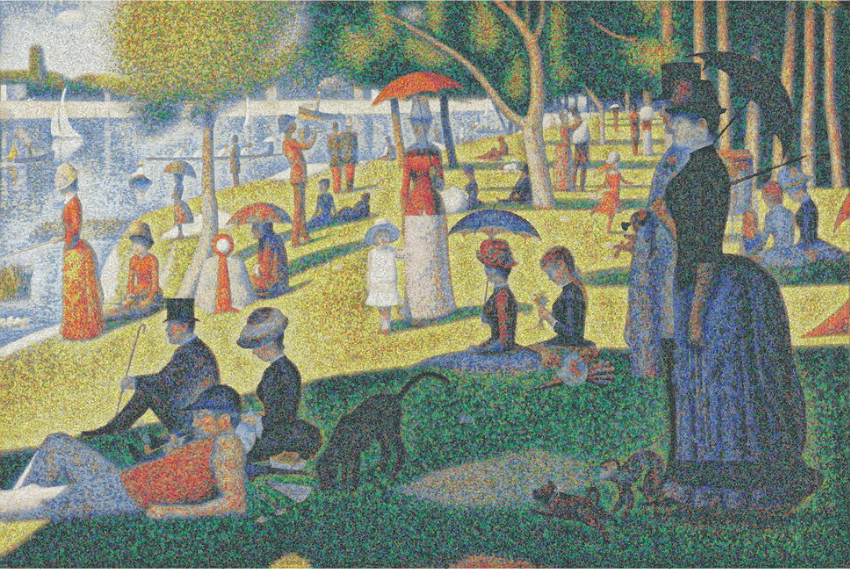
\includegraphics[width=\linewidth]{graphics/ChrisJordan_Numbers_OriginalView.jpg}
  \caption{Original view}
  \label{fig:ChrisJordan_Numbers_CloseView}
\end{subfigure}
\hfill
\begin{subfigure}{.47\textwidth}
  \centering
  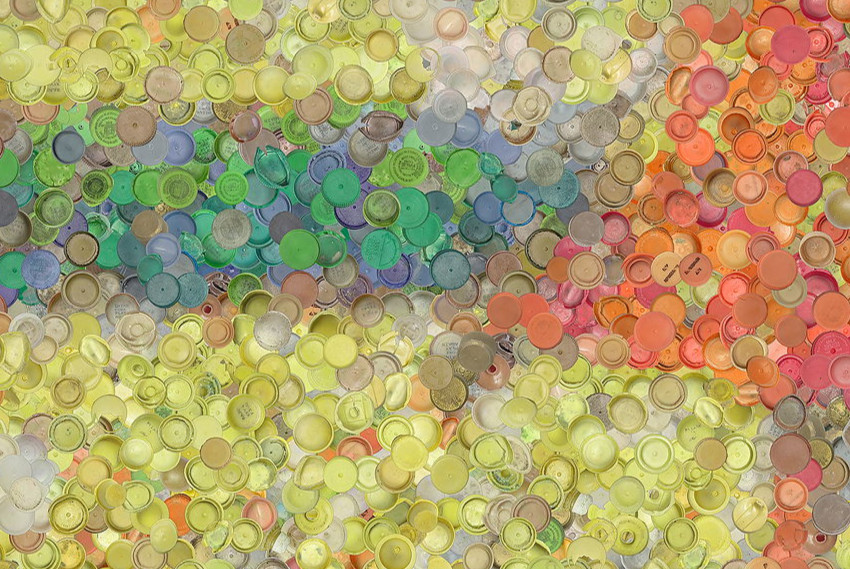
\includegraphics[width=\linewidth]{graphics/ChrisJordan_Numbers_CloseView.jpg}
  \caption{Close view}
  \label{fig:ChrisJordan_Numbers_OriginalView}
\end{subfigure}
\caption{Chris Jordan, Caps Seurat, 2011, 60x90" in one panel, and 88x132" in 3 panels}
\label{fig:ChrisJordan_Numbers_CapsSeurat}
\end{figure}

Chris Jordan creates digital photographic series that turns numbers to visuals. He provides a different way to understand the statistics and the missed reality of consumerism. He creates gigantic prints to express the numbers in a visual manner. He draws attention the global consumerism. The work reveals the reality that is hard to capture because of widespread of subject to the community and time.

Caps Seurat depicts 400,000 plastic bottle caps, equal to the average number of plastic bottles consumed in the United States every minute. It is one of the pieces of Portraits of Global Mass Culture by Chris Jordan is a series of work. In this series, he revisits the statistics of modern societies.  In Running the Numbers, photographer Chris Jordan attempts to convey the vastness of modern consumption by breaking down annual statistics into more graspable quantities depicted by clever visualizations made of individual objects or groups of objects that he photographs. “There’s a disconnect that happens when we assume we know what we’re talking about when we talk about hundreds of millions of plastic bottles,” Jordan says. “I’m trying to translate these numbers from the deadening language of statistics into a visual language that allows some kind of comprehension.” Many of Jordan's works are created from photographs of garbage and mass consumption Jordan uses everyday commonalities such as a plastic cup and defines the blind unawareness involved in American consumerism. His work, while often unsettling, is a bold message about unconscious behaviors in our everyday lives, leaving it to the viewer to draw conclusions about the inevitable consequences which will arise from our habits. He recreates the most remarkable artworks with combining bits of trashes as a mosaic. Here he draw attention to the our consumerism and express them numbers that are very big to understand. All the material that we have is trash to create this pictures.

%\summary{Analysis}
In fact, the work of Chris Jordan is a reproduction of A Sunday Afternoon on the Island of La Grande Jatte which is one of the most notable works of Georges Seurat who was acknowledged as the painter of a post form of Impressionism called Neo-Impressionism. The work accepted as a well-known example of pointilizm that is a technique of painting in which little, individual dots of color are applied in patterns to form an image. This method shows similarities with mosaics of ancient times and pixels of modern times. To make an work from bottle cups with different colors can be related to painting millions of small dots on a canvas. The shape of plastics cups similar to the dots painted onto the canvas so that there could not be a better example of reproduction.

Seurat spent over two years painting A Sunday Afternoon, focusing meticulously on the landscape of the park. However, in our age, it takes only one minute to create the bottle caps that form this painting. In this respect, it reveals the point where society reached.

Visuals of Chris Jordan are like modern versions of mosaics. In the age of mass production and consumption, the most readily available material is trash. It is free and available everywhere, produced every time. Trash has different colors, sizes, and shapes. Therefore, it is a perfect material to build sculptures from them. There is a great diversity of rubbish and offers new alternatives. Nothing is missing with the physical attributes of trash to create visual work.

% Here, sculptures from trash can be added.

% ARTWORK
% TEA BAGS
% FROM https://instagram.com/silvirub/, http://www.rubysilvious.com/363-days-of-tea
\begin{figure}[h!]
  \centering
  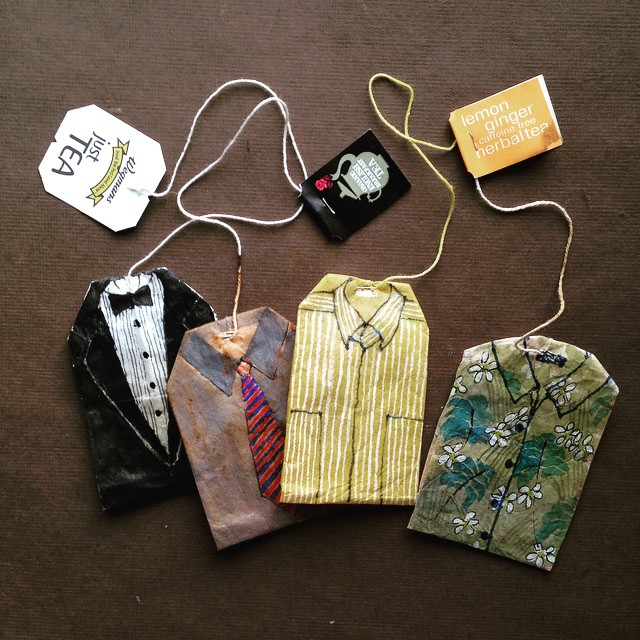
\includegraphics[height=6cm]{graphics/rubysilvious-teabag-Day169.jpg}
  \caption{Ruby Silvious, Day 169, 363 Days of Tea, 2015, Mixed media on upcycled paper tea bags, Dimensions variable}
  \label{fig:RubySilvious_TeaBag}
\end{figure}
  
Visual artist and graphic designer Ruby Silvious embarked on a quirky, personal experiment, set to last for 363 days. She decided to repurpose soggy and stained tea bags as unconventional, blank canvases, just waiting to be filled with her artistic expression. The project, entitled 363 Days of Tea, allows Silvious to challenge herself by transforming the recycled material with her intricate illustrations. The artist draws, paints, and forms collages on the salvaged tea bags. This project serves as Silvious’ daily journal, allowing her to record her thoughts and feelings by creating wonderful moody and whimsical designs on little teabag papers. Every day she creates a new piece that reflects her impressions in that moment. Endeavour of re-purposing recycled and found materials. 
%\todo{cite website}

%\summary{Analysis}
This work is for fathers day. Works of Silvious catch the important moments of days and can be as a diary (or a record of that moment and day). Trashes transformed to diaries. Trash is everywhere, already at hand. Small pieces of paper or packages are used as a canvas. 

% ARTWORK
% COFFEE CUP
% FROM http://www.gwynethleech.com/
\begin{figure}[h!]
\centering
\begin{subfigure}{.47\textwidth}
  \centering
  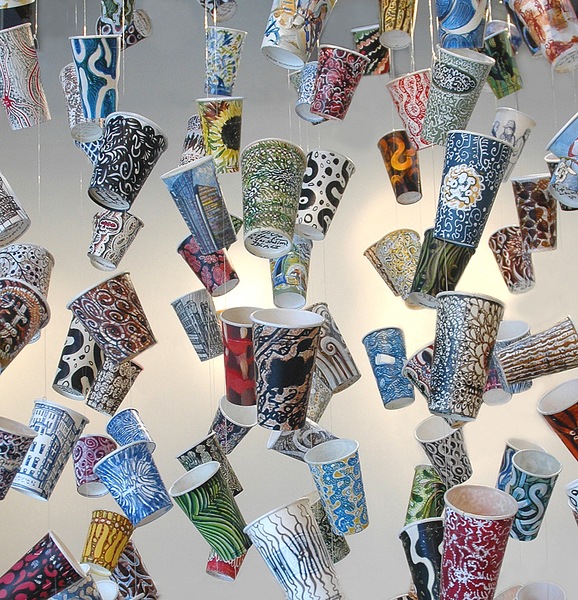
\includegraphics[width=\linewidth]{graphics/Gwyneth-Leech-cup5.jpg}
  \caption{Installation view}
  \label{fig:GwynethLeech_Installation}
\end{subfigure}
\hfill
\begin{subfigure}{.47\textwidth}
  \centering
  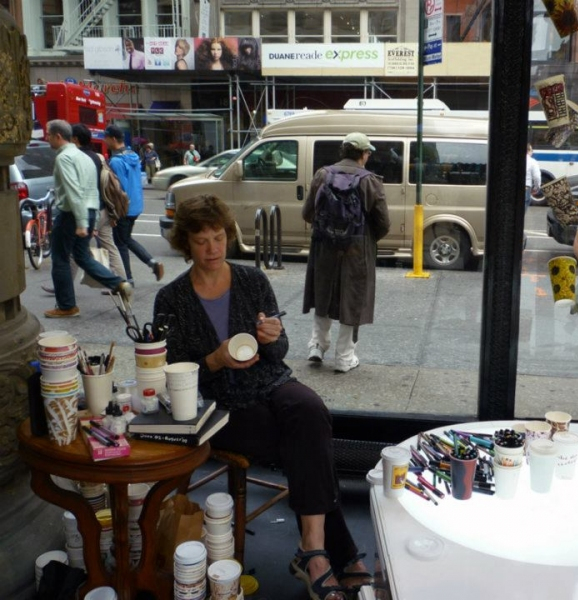
\includegraphics[width=\linewidth]{graphics/Gwyneth-Leech-cup3.jpg}
  \caption{Painting in the public}
  \label{fig:GwynethLeech_Public}
\end{subfigure}
\caption{Gwyneth Leech, 365 A Year in Cups, 2013, Mixed media on upcycled paper coffee cups, Dimensions variable}
\label{fig:GwynethLeech_CoffeeCups}
\end{figure}

She saves all of her coffee cups to use as "canvases" for making art. Transforms coffee cups that are no longer trash but a vehicle for art, ideas, conversation, and memories of a social moment upcycled from the detritus of our throwaway caffeine culture. She uses cups as a surface on which to draw and paint. Moreover, on the bottom of each one, She record the date, location, occasion and beverage consumed so that every hand-made cup artwork becomes the record of a social moment. Each cup is representing a daily caffeine break. The installation makes visible largely unconscious patterns of consumption; this is what one simple take-away purchase looks like over the course of three years, this is what would usually be thrown away. It can be seen as a measure of time gone by, of money spent, of space to be taken up in a landfill. However, as I upcycle each used cup into an artwork, it becomes the measure of other things as well: an artist's regular habit of generating new ideas, a diary of time spent with friends and colleagues, and the cumulative positive effect of doing something small and manageable every day. There are different versions of it. Paintings on paper coffee cups displayed in open window spaces. She publicly draws their cups (the cup art window installation and public drawing project were on view repeated showed at many places and date. During public drawing projects, she draws with other people. Moreover, so. Buying a beverage is a daily event for Leech (and also many people. These coffee shops all around the world. As she drinks her coffee in the public, she also publicly transforms its cup.
%\todo{cite her website}

%\summary{Analysis}
She is inside of glass window not white, isolated cube. Glass window provide her to be close to public space. As she drinks her coffee publicly, also paints them publicly. 
%\todo{related with Liz Parson's argument: practice of trash to durable.} 
There is no difference between them, and also they should not be separated. By showing her practice publicly, she encourages other people in order to reconsider trash as a resource to make something. Further she is not only transforming her trash, it is everybody's trash because of everyone uses it.

These three artists mentioned here use disposable items to make their art. Their approach bring another dimension to criticize (or see) the disposable items. New things can be built from them. They can be used for new purposes.

Throwaway culture is a way of producing trash. It is a behavioral pattern, an approach to objects and commodities. Some artists develop different approaches to them. In this type of culture or behavior throwing them is a natural act and promoted. Consumption and wasting things are encouraged. On the other hand, there are examples of saving everything instead of wasting. In the work of Song Dong, "Waste Not" thousands of domestic objects are exhibited. They are owned by his mother and saved for later use. His mother lived a great depression in China, suffered from poorness. She developed the habit of saving things. After died of her husband this habit reached to extreme levels. She saves every tiny little thing. For her trash becomes an essential part of her life. In fact, it not is hard to say that preserved these things are not useless or worthless. She establishes a different relationship with these used objects.





%
%
Trash is much more than what people want to discard. Characteristic of people and societies can be understood from their produced trash.


%\summary{TRASH and POTRAIT OF PEOPLE} 
Trash is a reminder of consumption and production activities. In other words, trash is bound to them, and every different of them leaves a diverse range of trash that exposes its type of action. Trash tells about societies' choices. What is being left is one of the key things to realize what kind of people, society, action produce it. At one side trash is a produced thing and  What people consume is tells many things about them (their choices, possessions, etc.) 
%\todo{ref.}
. As scholars mentioned that throughout the discards of someone else many things can be understood. They are end product of people activities, and it can be traced through the discard and garbage. It is a great example of the approach to the trash is relative and changes from people to people.

\begin{figure}[h!]
  \centering
  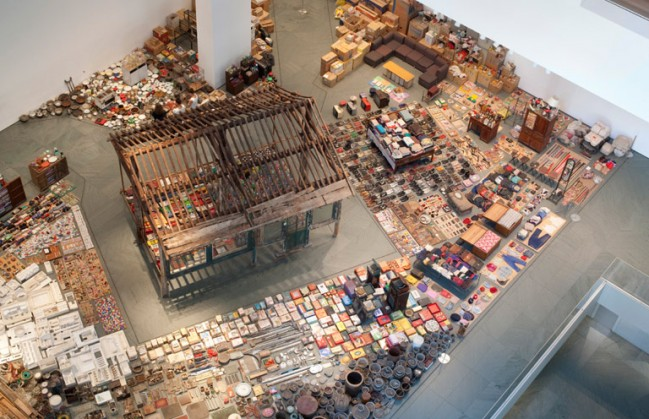
\includegraphics[height=6cm]{graphics/SongDong_WasteNot.jpg}
  \caption{Song Dong, Waste Not, 1990}
  \label{fig:SongDong_WasteNot}
\end{figure}

"Waste Not" is an exhibit by Chinese artist Song Dong that displays over 10,000 domestic objects formerly owned by his late mother, who refused to throw anything away if she could possibly reuse it. 

Song’s mother, Zhao Xiangyuan (1938–2009), was typical of the generation of Chinese who lived through the hardships of the Cultural Revolution in the 1960s and 1970s abiding by the dictum "wu jin qi yong" (waste not). As a result, all commodities owned or collected stockpiled and preserved as protection against future hardship, even in the face of improving economic conditions.

Waste Not is an installation exhibited different locations of the world. This work is a collaboration with the artist’s mother.

Like many other Chinese at the time, Zhao adopted the habits of frugality and thrift in order to make the best of what little she had. Song recalls that when he was a child, "my mother always brought scraps of fabric to make clothes, because they didn't need to be purchased with the government-distributed clothing coupons." She continued to collect them even in better times because she feared that the shortages might some day return, seeing the habit of "waste not" as a fabao – literally a "magic weapon" to guard against a return to poverty.

When Song's father died suddenly in 2002 his mother suffered an emotional breakdown and her habit of holding on to things was taken to extremes, with every possible space of her tiny house crammed with thousands of domestic odds and ends. Song Dong and his sister Song Hui attempted to tidy up for her, but this led to conflict, as Zhao opposed their efforts to dispose of things that she saw as potentially useful. Song eventually came to understand that, as he puts it:

\begin{singlespace}
\begin{quote}
My mother's need to fill space with daily-life objects resulted from a need to fill the emptiness after my father's death. I recognised that in this era of transition, a person could live through several different lives in just one lifetime. In the wink of an eye, one's life could undergo great changes causing deep divisions between old and young.
\end{quote}
\end{singlespace}

Everything that are exhibited here is different than presented on supermarkets. They are not new and not for sale. They represent a way of life. It is common that the exhibition (museum) of famous people's possessions but this work is separated from them as showing ordinary people's objects

For most of people living in western modern societies it is unimaginable to live with all of these items together. However, for Chinese who are faced with same struggles share the emotion and  comment as "It's not [only] your home, it's my home."

Jane Alison, senior curator at the Barbican, said that Waste Not helps us to understand the reality of Chinese history and culture in the 20th century in a way that newspapers can't.

% TODO need relocation
% FROM Culture, Values, and Garbage, Encyclopedia 
%\comment{INTERACTION WITH GARBAGE. VALUE SYSTEM, DECIDING TO GARBAGE.}
%\paraphrase{"The Trash Talk project emphasizes the complex, yet overlooked, relationships that garbage and people share. In terms of their relationship to garbage, all people interact with it on two levels. One is a material connection, indicative of the physical and sensory contacts that people have with garbage. In some households, this connection begins with an individual removing an item from packaging, disposing of that item in the kitchen receptacle, placing that item and others into a larger bin, taking that bin to the curbside, and then the material connection ends. Others, including workers in sanitation plants and recycling centers, then continue a material connection with the garbage, but the material connection of the consumer and the garbage ends with the bin on the curbside. The second connection that people maintain with garbage is an ideational one. Unlike the material one, which is manifested in things that can be touched, moved, and sensed, the ideational connection operates on the level of cognition. The differentiation of an item of value from an item of trash, for example, has nothing to do with the material principles of the object. Instead, humans determine whether the object is of value or whether it is considered trash. The decision of whether an individual decides to dispose of a broken radio or to consider it an heirloom to be kept is highly subjective and rooted in the value systems of a culture." "After the item is eaten, the individual has to decide what to do with the remainder, such as the leftover package. The package might be reused, re-purposed, or recycled but, most likely, will be disposed of in the trash." \cite{lukas2012culture}}



% TODO need relocation.
% FROM Garbage in Modern Thought, Encyclopedia
%\comment{CATEGORIZATION.} \paraphrase{"Garbage is categorization, according to Susan Strasser." "In recycling programs and in places of refuse disposal, items of trash are categorized depending on their potential value, possible environmental harm, or time of decay. Consumers have become accustomed to the categories that are often applied to garbage. Many cities require people to dispose of their garbage in an orderly fashion---perhaps separating wet household waste from dry---and recycling programs ask individuals to divide their recyclable items into sets (such as plastic, glass, aluminum, and paper). Garbage is an illustration of how humans use mental categories to order the material world." \cite{lukas2012garbage}}

% TODO need relocation.
% Garbage is universal.
%\comment{NO VALUE, UNIVERSAL} \paraphrase{"According to John Scanlon, garbage is indicative of a separation of the world---the desirable from the unwanted. Michael Thompson uses the riddle of the rich and poor person’s approach to snot (one keeps his in a handkerchief, the other disposes of it with a tissue) to underscore the curious ways in which garbage is connected to the issue of value. While garbage is universal---all societies, extinct and extant, have produced or produce garbage--- the conditions under which garbage is understood are culturally determined. Many non-Western societies attach a much greater value to items after they are discarded. In the United States and many other nations, garbage often results not because something no longer has utilitarian value but because the item in question is defined as something of no value. Thus, garbage is not only an objective condition of material culture, but also a subjective one of mentalist culture. People define what is trash and what is valuable." \cite{lukas2012garbage}}





%
%
%\summary{Garbology}
Garbology is a study of waste as a social science. Applying methodologies of archeology to the human debris. 

Weberman infamously used techniques of what he deemed garbology to uncover what he saw as the essential nature of people. He once said, perhaps indirectly referencing Jean Brillat-Savarin’s quote about food, \quotes{You are what you throw away} \citep{lukas2012garbage}.

% Garbology, from Encyclopedia, Abhijit Roy
The field of garbology involves the study of refuse and waste. It enables researchers to document information on the nature and changing patterns of modern refuse, hence assisting in the study of contemporary human society or culture \citep{roy2012garbology}. According to the Oxford English Dictionary, the term was first used by waste collectors in the 1960s. Weberman popularized the term in describing his study of Bob Dylan’s garbage in 1970. It was pioneered as an academic discipline by William Rathje at the University of Arizona in 1973.
%roy2012garbology

The work of archaeologists such as William Rathje and Cullen Murphy has offered significant insights into the relationship between archaeological artifacts and garbage, exploring the function of trash as a resource for understanding the cultural and social practice. At the same time, thinkers such as Zygmunt Bauman and Giorgio Agamben have shed light on the fate of the human being as a wasted or discarded element in discourses of socio-political hygiene \citep{pye2010trashculture}. 

%\todo{transition required.} 
With the help of mentioned understanding of trash, what can we see the work of arts?

\begin{figure}[h!]
  \centering
  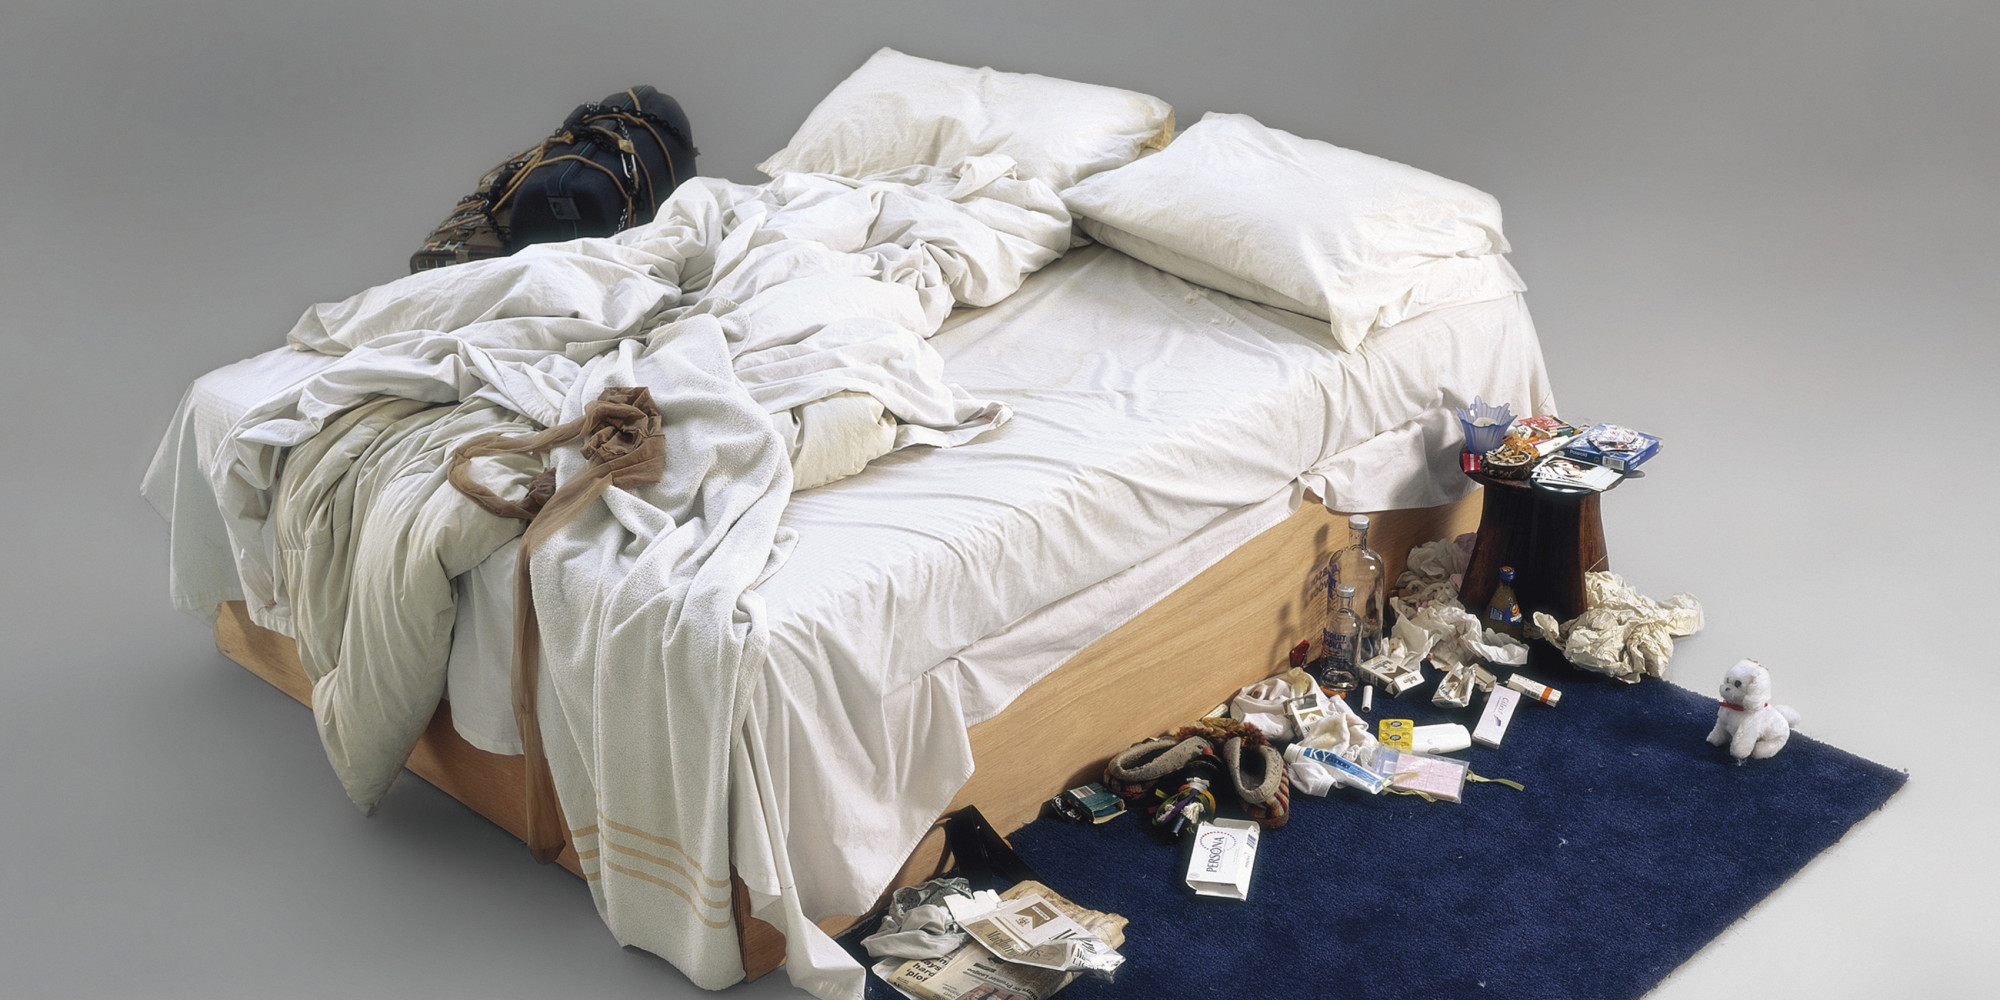
\includegraphics[height=6cm]{graphics/tracey-emin-my-bed.jpg}
  \caption{Tracey Emin, My Bed, 1998}
  \label{fig:TraceyEmin_MyBed}
\end{figure}

Tracey Emin puts her private life to the public. The work, which Emin now describes as a portrait of a young woman. Around her, there are pieces of junks speared all over the room. We can understand from her junk what type of life she has. We enter the world of the artist through her trashes.

% From wiki
Every detail of her private life is presented through her bed. The idea for The Bed was inspired by a depressive phase in the artist’s life when she had remained in bed for several days without eating or drinking anything but alcohol. The sensation of depression leading to disarray and detritus is not wholly unfamiliar to many people, and The Bed therefore enforces the communicative power that Tracey Emin seeks with her work. The artwork generated considerable media furor, particularly over the fact that the bed sheets were stained with bodily secretions and the floor had items from the artist's room, such as condoms, underwear with menstrual blood stains, other detritus, and functional, everyday objects, including a pair of slippers. The bed was presented in the state that Emin claimed it had been after languishing in it for several days; at the time she was suffering suicidal depression brought on by relationship difficulties.

It is a realization what she did during her depression time. It perfectly represents her condition during those days. It can be understood that trash is part of our life. Things that are exhibited in this work are part of her action. She created them and later through them in the mind of people the condition and life of Tracey Emin are recreated. 

% Independent http://www.independent.co.uk/arts-entertainment/art/reviews/tracey-emins-my-bed-at-tate-britain-review-in-the-flesh-its-frankness-is-still-arresting-10144882.html
You can interpret it as an uncompromising self-portrait of a woman at a time of emotional trauma – or as a turbulent still life – but it is still a bed and all that a bed symbolizes and encompasses: sleep, sleeplessness, sex in all its manifestations, birth, death and dreams.

Beds are not just for sleep. Especially for the ones that have small rooms and spaces bed becomes a life space. I have also experienced such a thing at boarding school and university dormitory for total my eight years. Having tight space sometimes bed becomes a place for studying and reading. Sometimes it was used to dry the clothes. It is more than sleeping and provide place for other activities.

% tracey emin joseph beuys arasında bir ilişki var. sanatsal eylem ve kalıntı olarak bakıldığında.

% Aslan yattigi yerden belli olur.





%
%
\section{Zizek's Approach to Rubbish}
Last decades there is an increasing attention the ecology and rubbish. Global warming is one of them, plastic pollution on the oceans also is part of it. These types of news and talks increasingly find a place on media more and more. At this stage, Zizek comments on ecology and trash conversely.

\begin{singlespace}
\begin{quote}
In the late twentieth century, in the context of increasing environmental awareness, this consciousness has altered yet again, and waste has been revalued and recoded from rubbish to recyclable resource, it has moved from the bin to the compost heap, it has insinuated itself into our lives in different ways and with different effects \citep[5]{hawkins2005ethics}.
\end{quote}
\end{singlespace}

In the documentary film Examined-life Zizek dressed as a sanitation man discusses ecology in the middle of a dump in London. His part starts with these sentence: \quotes{This [dump] is where we should start feeling at home}. The place where he talks is a site for depositing people's excess and unwanted material. It is a place of out of sight.

He draws attention that the thrown out garbage only disappears from people's living environment. Particularly discarding it is an action of escape from the unwanted. However, it still exists in reality and waits at somewhere else. In other words, it does not disappear, moves away.

According to Zizek, the way of approaching ecology is problematic in current societies because of accepting nature as a balanced, and harmonious. He claims that it is ideological in the sense that "wrong way of thinking and perceiving reality". The meaning of ideology is here mystification of real problems. He claims that one of the key mechanism of ideology is temptation of meaning. In other words, people search for meaning when a terrible event happens in order to make it easier to accept. He opposed the notion of the existing world is in the best possible state and that humans disturb nature. According to him, nature is not an organism in balance that humans exploit, but rather a series of "unimaginable catastrophes" by asking the question what type of disasters would happened on the earth to compose oil that is a significant source of energy. Zizek asserts that ecology will slowly turn to a conservative ideology that is a kind of an unquestionable highest authority. Its voice is like "Do not mess with D.N.A. Do not mess with nature". In the light of these arguments instead of talking from an authoritarian high ground, he suggests that to find poetry and spirituality in the dimension of rubbish people create. He thinks that that is the true love of the world by asserting that "love is not idealization." Therefore, that is the reason why he thinks that a dump is a place that people should accept it as a home. 

In the light of Zizek's arguments ecology is not an appropriate point (or enough) to approach trash. He points out the need for the new approach to trash. This new approach should not idealize it. At this point where the practices of art gains importance to establish new understanding of trash.

Not every act of transforming trash is not related to ecological concerns. Artists are not trying to save the planet earth. Beyond ecological concerns, they are attempting to find new ways to look and live with trash. 

Some artists turned to trash into site-specific sculptures that are more than trash heap after their intervention. Not discarding but bracing our attitudes turned them to a something that worth it to watch and think about it. (Converting what we create harmonious with the existing system. Because it is not possible to think that nature will live harmoniously with what we created. The more reasonable idea will be we will live harmoniously with what we create.) Turning trash to things that can be lived together.

%Beyond the ecological problem, there are different sides of it. Different readings can be added to the topic. Adding spirituality and new aesthetics dimension to the topic. 

The idealization of nature is problematic. Loving nature is loving trash. Live with trash. Do not see it as trash. Then the question is How to love trash? How to live with trash? Think beyond the common perception. Do not consider it as abject, disgust. Can live with our trash enrich (our perceptions, abilities)? How not to see them as trash and useless? Can it be possible with art?





%
%
\section{Rubbish Theory}
Objects have a lifetime similar to humans, and they do not remain same through that time. They move around, and their value, usage, location change constantly. During their lifetime objects may circulate different markets and values systems such as economic, social and aesthetic. Especially these cycles have picked up speed with the advent of consumer culture. For instance, most recent technological gadgets become obsolete within two or three years. Firsthand, secondhand and even trash is exchanged among not only people but also countries. People from other cultures and understanding interpret objects differently. They often are not aware of their initial and intended usage. They find new original purposes and meanings. Therefore, objects turn different items in their hand. Anthropologist Sidney Mintz (as cited in Susan Strasser) writes that "I have seen automobile bearings fashioned into portable vulcanizing kits; bits of toothbrush handles used as 'jewels' for rings, and ordinary tin cans turned into simple kerosene lamps." As it can be understood that objects function and value are transformed by relocation and revaluation of objects from one place to the other or one discipline to another. 

In ‘The Social Life of Things’ Appadurai (1986: 3) highlights that "commodities, like persons, have social lives." As such, Kopytoff wrote, the biography of an object was considerably similar to that of a person: occupying different positions, leading diverse careers in the course of different periods between a beginning and an end, being defined by different regimes of value that are both economically and culturally inscribed. Appadurai focuses on the "commodity potential" of things and asserts that "things can move in and out of the commodity state, that such movements can be slow or fast, reversible or terminal, normative or deviant" (1986: 13). However, one can ask that what are these commodity states and does anything exist between them? Thompson’s Rubbish Theory fills this gap.

Thompson observes the creation and destruction of value in man-made objects, cultural artifacts, and ideas. He notes how an object’s economic and cultural value diminishes over time rendering the objects worthless or redundant and how others value increases overtime. In his notable Rubbish Theory, he declares three object states; transient (normal state, decreasing value, circulating), durable (permanent, increasing value, removed from circulation) and rubbish (zero value, will be destroyed or reinvested for economic and social value). The transient represents the common state of objects that are lessening in value and have limited life period. A used car can be an example of transient state. On the contrary, the durable objects increase in value over time and have (ideally) infinite life spans. Antiques and objects in museums can be an example of durable. This theory gives rubbish a key role between transient and durable. 

% TODO Bu nereden
Rubbish is, by definition, an object that is not or is no longer, owned by anyone, which falls outside all categories of economics, culture, and social control. As one of many things on the garbage heap, a discarded object even tends to take on a negative value as something unsanitary, dangerous. The socially constructed value of the object has shifted over time from its finite life span of usefulness and meaning to a timeless and valueless of socially sanctioned rubbish. 

The potential of the discarded thing also relies on its status as a thing approaching a zero point of value. In other words, it has reached a point in transition between the world of the functioning, the useful and visible, and the realm of the invisible, the non-functioning and empty. As Michael Thompson’s Rubbish Theory suggests that rubbish is both ready for the disappearance and yet ripe for reinvestment, reinterpretation or revaluing. Trash as a state of being flexible is ready to transformation.

Similar to Žižek's claim that is "trash does not disappear", Thompson notes that "in reality ... [trash] just continues to exist in a timeless and valueless limbo, where, at some later date (if it has not by that time turned, or been made, into dust) it has the chance of being discovered."

Thompson argues that rubbish represents an important possible ‘in-between’ category in a ‘region of flexibility’ which is not subject to the same control mechanisms of the valuable and socially significant categories of transient and durable. Therefore it ‘is able to provide the path for the seemingly impossible transfer of an object from transience to durability’ (1979: 9) he further suggests that ‘a transient object gradually declining in value and in expected life span may slide across into rubbish’ (1979: 9) where it has the chance of being re-discovered, brought to light or cherished once gain. Figure X demonstrates the possible paths an object may take (from transient to rubbish and from rubbish to durable).

\begin{figure}[h!]
  \centering
  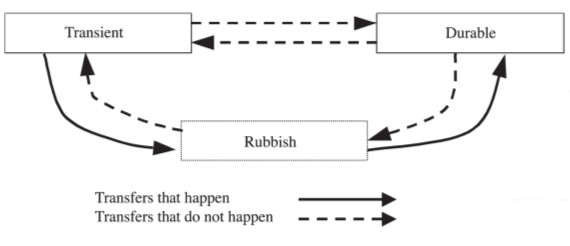
\includegraphics[height=4cm]{graphics/rubbish_theory.jpg}
  \caption{Thompson’s Rubbish Theory}
  \label{fig:rubish_theory}
\end{figure}

The transitions between these states defined as follows: from transient to rubbish (transient -> rubbish) and from rubbish to durable (rubbish -> durable). 

To illustrate rubbish theory the series of compression by French sculpture César can be analyzed in the context of it. His early work is composed of soldered and welded metal as well as junk materials. In 1960, Caesar discovered the hydraulic press that is capable of compacting scrap metal (especially car bodies) during on a visit to a scrap merchant in search of metal. He admired from the hydraulic crushing machine in operation and started to experiment with it in his sculptures. The machine is used to compress the metal items in order to gain from space. His first three automobile compression exhibited at Salon de Mai in 1960 and bring him a supportive fame. Later Viscountess Marie-Laure de Noailles who is important figure of these ages, gave him her Zim model car to compress. It is 
% http://www.sothebys.com/en/auctions/ecatalogue/2015/art-contemporain-pf1515/lot.6.html
"a revolutionary artistic gesture then, but also a strong political gesture, right in the middle of the Cold War; César having chosen to lash out against a Zim, a jewel of the Soviet automobile industry commissioned by Khrushchev at the beginning of the 1950s to compete with the Cadillac." Additionally car was one of the most desired possessions of people in 20th century. Through the eyes of rubbish theory it is a transient object and after the intervention of artist, it is transformed into an artwork that preserved in the collection of Museum. In other words, it switched to durable category by interestingly trashing it. 

\begin{figure}[h!]
  \centering
  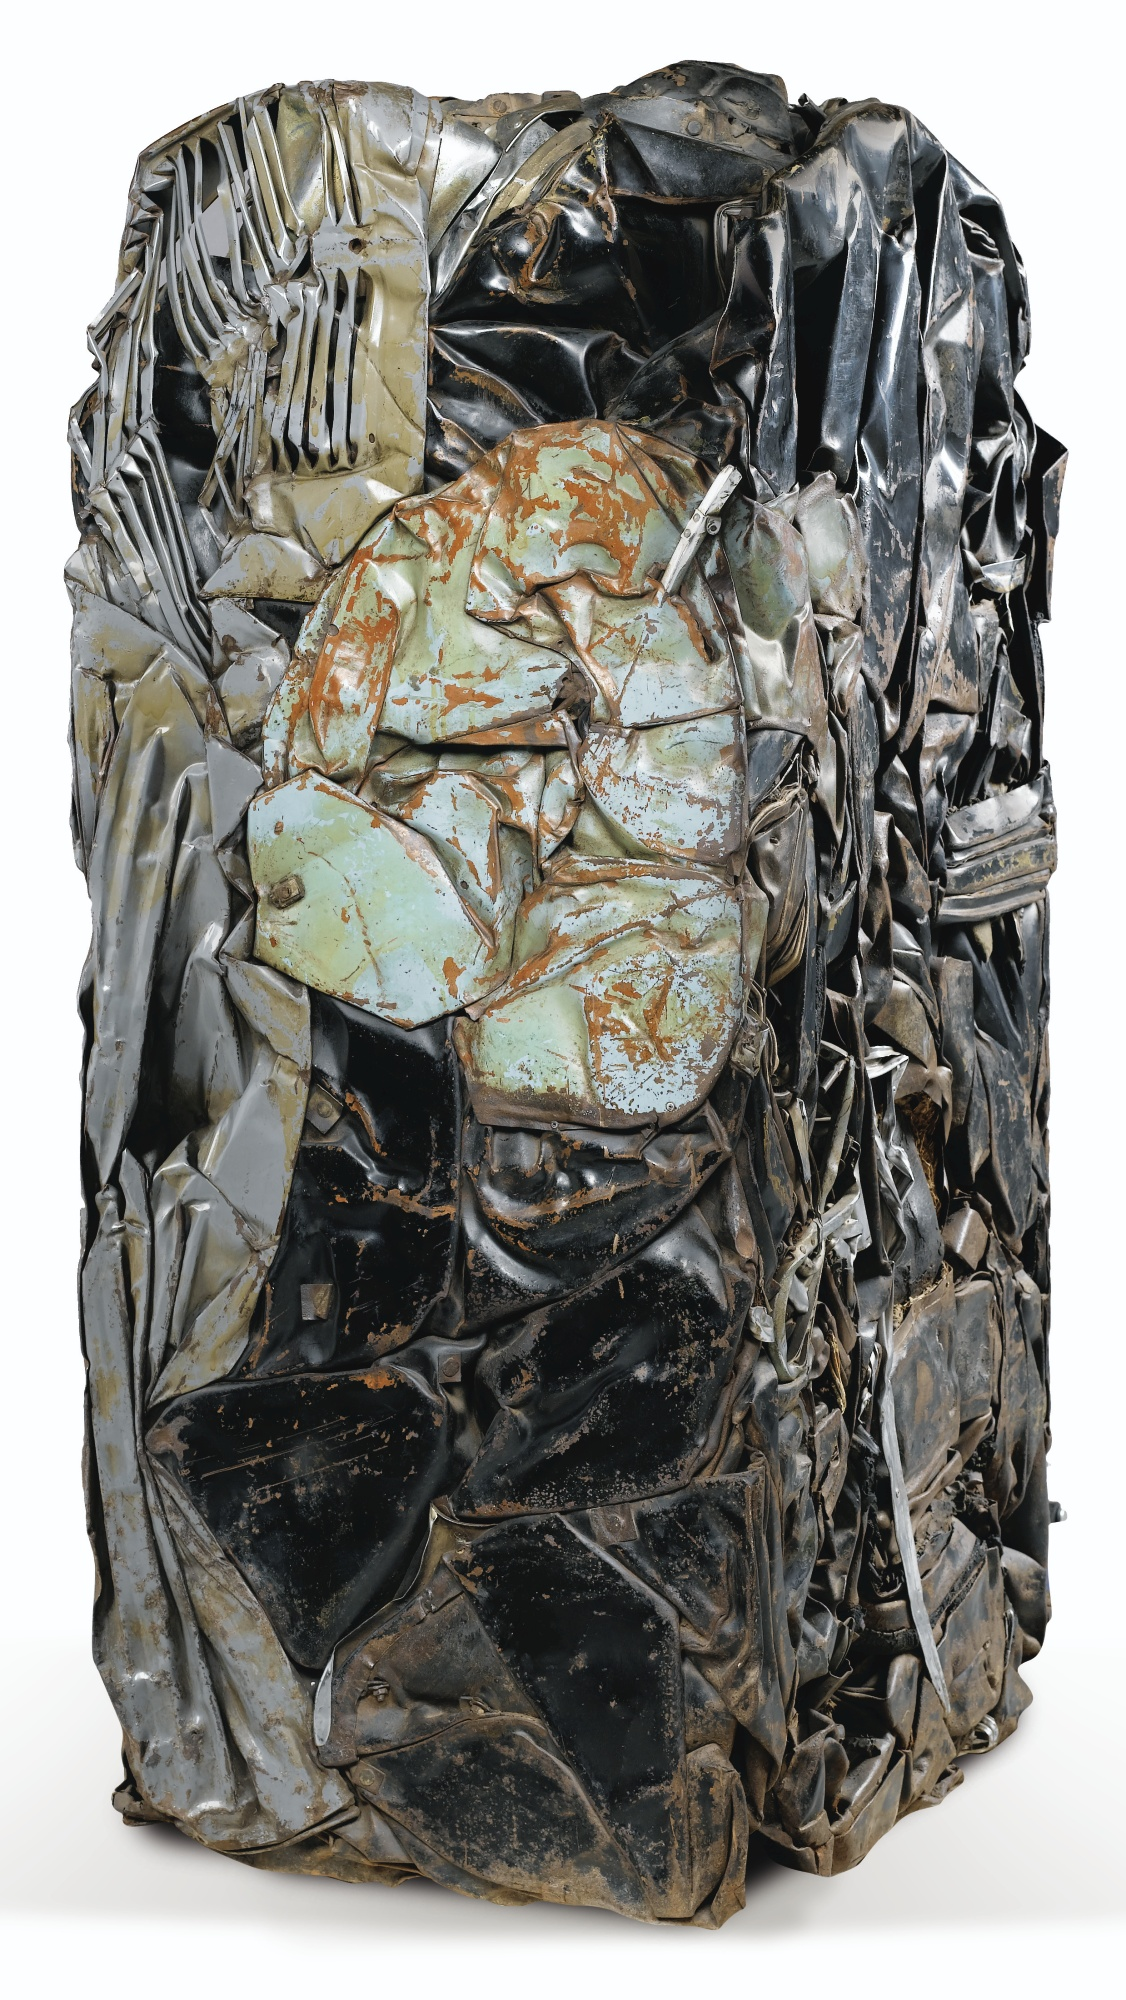
\includegraphics[height=6cm]{graphics/Cesar_Zim.jpg}
  \caption{César, Compression Zim, 1960-1961, 157 x 82 x 64 cm}
  \label{fig:Cesar_Zim}
\end{figure}

Although Thompson is quite successful describing states of objects, claimed transitions between states in the theory have some problems. Thompson label some transitions as possible and the others as impossible. He only allows movement of goods from transient to rubbish, and from rubbish to durable. Movement in the other directions, from durable to either transient or rubbish, does not exist in this system. However, Duchamp's notable ready-made "Fountain" is one of the examples outside of the defined transitions.

\begin{figure}[h!]
  \centering
  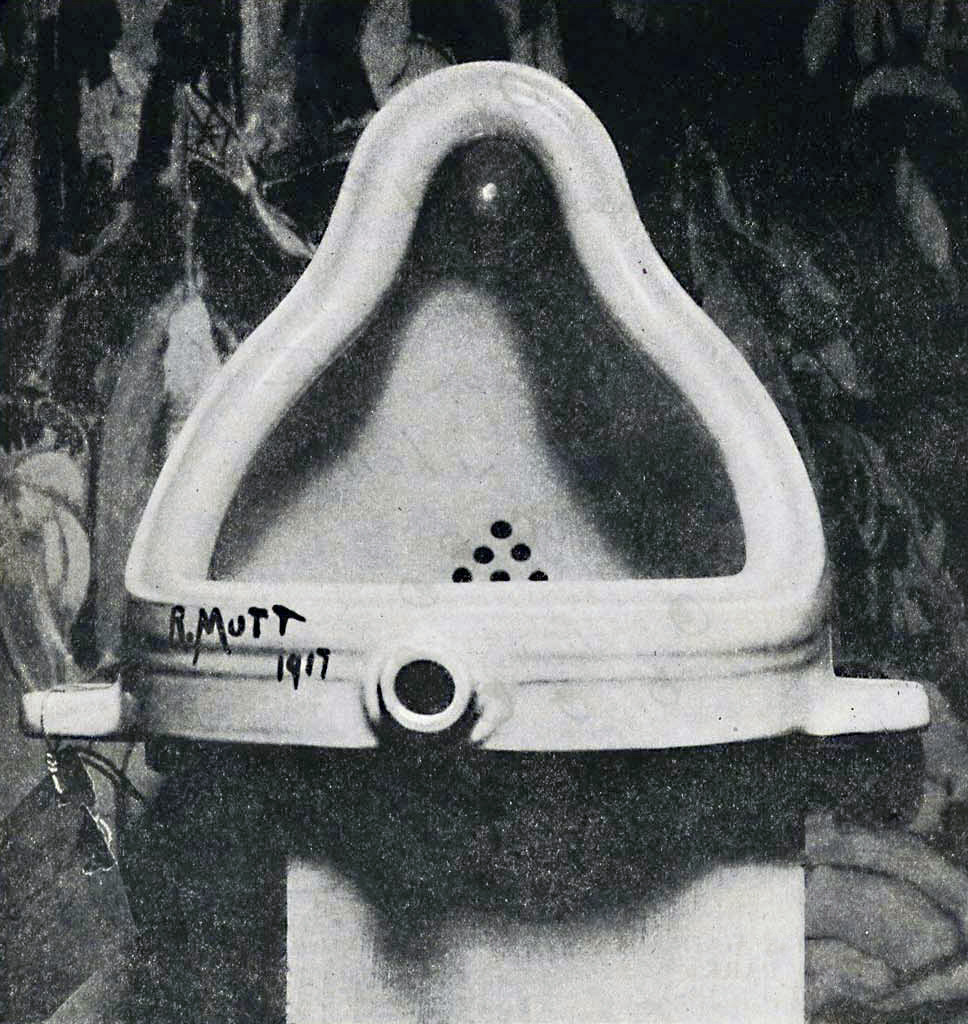
\includegraphics[height=6cm]{graphics/Duchamp_Fountaine.jpg}
  \caption{Marcel Duchamp, Fountain, 1917}
  \label{fig:Duchamp_Fountaine}
\end{figure}

Fountain is a 1917 work produced by Marcel Duchamp, who is notable member of provocative Dada movement. The piece was an industrial porcelain urinal, which was signed "R.Mutt". Submitted for the exhibition of the Society of Independent Artists, in 1917, Fountain was rejected by the committee, even though the rules stated that all works would be accepted from artists who paid the fee. It is considered one of the major artworks of the 20th century because of challenging the existing understanding of art. Duchamp used already existing fabricated ordinary urinal to express his ideas by challenging existing way of art making which requires efforts of the artist. It forces to the limits of the language of art and perception the art. To understand his works requires shift inside of the peoples mind. For him, the idea is important rather than the object. He also criticized the position of artist by signing urinal as "R.Mutt" who is actually not exist. In the editorial The Blind Man summarized this work as follows: \quotes{Whether Mr. Mutt with his own hands made the fountain or not has no importance. He CHOSE it. He took an ordinary article of life, placed it so that its useful significance disappeared under the new title and point of view – created a new thought for that object} \citep{duchamp1917mutt}. To debate all the aspects of this work is not possible with the scope of this thesis. However when it is analyzed through the frame of rubbish theory, urinal a transient object turned to durable objects that are exhibited by the intervention of artist. Urine titled as "fountain" is still functional and have a place in the market. In another word, it is not rubbish.

%\todo{bir conslusion lazım buraya.}

% TODO move to conclusion.
%Rubbish theory suggests that value emerges through people ways of seeing, and their category membership determines the way people act towards them. Similar to X (as indicating that scholars agree on this argument.) 

% TODO move to conclusion.
% \paraphrase{Michael Thompson’s study Rubbish Theory elaborated an understanding of rubbish as part of a flexible and shifting system of value construction, underlying notions of innovation, creativity, and social status.} \todo{ref. from Trash Culture} \paraphrase{It is clear that one man's rubbish can be another man's desirable object; that rubbish, like beauty, is in the eye of the beholder \cite[97]{thompson1979rubbish}.}





% TODO relocate
% From "Trash Moves On Landfills, Urban Litter and Art" by Maite Zubiaurre
%\summary{Moves} 
%\paraphrase{Below part explains journey of trash in different steps/stages. Object moves and trash also moves. How is it life of trash? This part explains life of trash. How does it intersect with other people in which places? This part also can be understand by pointing out different part of it with detailed explanation. For example an artist collect from trash from streets and the other one goes to the (For example Vik Muniz) landfill. In other words there are different places to touch on trash. Every place generates different story? Or to understand it more deeply it covers different part of it. Or provides ideas about it. Lots of people touches it from philosophers to artist. Also in the later parts it draws attention to them.}

% TODO relocate
%\summary{Moves}
%\paraphrase{Trash moves, all the time. It becomes a steadily growing heap of clutter behind closed walls, accumulates and festers under tight lids, travels from a small trash can in the kitchen to a large one on the curbside, joins other people’s rubbish when the garbage truck arrives, drives to the transfer station, where it circles around on conveyer belts, bids farewell to recyclable or composable goods, is loaded (if declared useless: the ultimate trash) into yet another garbage truck, or barge, or even train, until it arrives at its final destination: a sanitary landfill. Even in the landfill, it does not remain still. Monster "waste handling dozers" move rubbish around, compact it and press it against the soil. More importantly, they incessantly “sculpt” refuse with their huge shovels and caterpillar wheels, making sure the garbage mound does not tip over to create a fetid avalanche. When night falls, and the trash load of the day finally disappears under a thick layer of mud, detritus still moves: once underground, it settles differently, and decomposes at a different speed, thus continuously altering landfill topography: where there was an even plateau, now there is an abruptly descending slope, and a valley; and where there was a perfectly smooth road, now there are deep crevices in the pavement. This is how trash moves. But\ldots who moves on trash? In the United States, it is mostly big-wheeled machines, an industrious army of giant yellow insects busying themselves on a heap of rubbish. In Latin America, it is mostly people. People who hand-pick garbage, who build their shacks on densely compacted trash layers, and who, day in and day out, eagerly throw themselves into the boisterous cascades of fresh debris falling from garbage trucks. In many of the garbage dumps around the world, scavenging becomes a steady job. \quotes{Garbage properly \quotes{stored} and put away brings peace of mind, as do corpses boxed and buried, or criminals confined to a cell.} And thanks to Art: for Art shows how trash--even the one that stops moving, and particularly the one that lies squished, squashed, and weathered, almost fossilized, on the ground---has the potential to move: to move us, that is. (through the works of Filomena Cruz's photographic series “Road Kill”)}

% TODO relocate
%\summary{Categorization of waste} 
%\paraphrase{Douglas argues that our classification of dirt lies not with what objects are but where those objects are. (Think that the transformation process. Previous argument support that the transformation of trash is possible by changing the place of them. In other words removing them from landfill and waste bins to the book selves accomplish to transform trash.) ‘Dirt’, writes Douglas, ‘is the by-product of a systematic ordering and classification of matter, in so far as ordering involves rejecting inappropriate elements’. For Douglas dirt is a spatial problem, a question of not what stuff is but where it is.} \todo{Reference, (Waste by William Viney).} 

% TODO relocate
%\paraphrase{“Dirt”, writes Douglas, “is the by-product of a systematic ordering and classification of matter, in so far as ordering involves rejecting inappropriate elements.” Dirt is only dirty in certain places, when it is out of its correct position. Just as faces, for example, is considered dirty when it is in our kitchens but not when it is in our bodies, so it is that our classification of waste depends on the location of objects.}  \todo{Reference, (Waste by William Viney).}

% TODO relocate
%\paraphrase{Waste is “matter is out place”, a definition first given by Lord Palmerston in the mid-nineteenth century and incubated by the British anthropologist Mary Douglas, in her book Purity and Danger.}

% TODO relocate
%Trash is something that is out of sight, out of mind. Paid little attention to them and only catches attention when it is in wrong place. It is an unexpected object for people. Therefore transformation of it can create powerful and suprising effect onto the people. 

% TODO relocate
%\paraphrase{Thompson comments that we only notice rubbish when it is in the wrong place, and highlights the embarrassment and anxiety that mis-placed rubbish, or rubbish which has found its way in to the wrong place can cause ‘Something which has been discarded, but never threatens to intrude, does not worry us at all.’ (1979: 92) but rubbish in the wrong place is ‘emphatically visible and extremely embarrassing’ (1972: 92). (Further there is similar analogy at Waste and Want. The author give the example of shoe and claim that thrash is relative. The shoe on the dinner table is something disgusting but in the foots is not at like that.) Rubbish objects are things that are no longer used or loved or cared for and often no longer seen. Rubbish objects linger on the periphery of our lives, in the back of the drawer, bottom of the wardrobe or cupboard, corner of the garage or garden shed gathering dust. (Summary From Liz Parsons.)} 









%
% TODO move it to the art chapter and discuss it with the found photos.
%\subsection{Rubbish Theory in Practice: From Rubbish to Durable}
%\paraphrase{In rubbish theory beyond the objects states how it happens transition of objects in practice is missing and Parsons fills this gap by claiming that transition from rubbish to durable are possible with finding objects, displaying objects, re-using objects \cite{parsons2008thompsons}.} (finding paper, transforming to notebooks and giving away them to create an opportunity to be displayed different location and times.) 

%Three such sets of practices are explored below, they include: finding objects, displaying objects and transforming and re-using objects. It is argued that each of these sets of practices changes the way we view an object moving it from being seen as a ‘rubbish object’ of no value to a ‘durable object’ of increasing value.

%\textbf{Finding Objects:} One key way in which objects may slide from the category of rubbish to durable is through the act of finding. Indeed, Gabriel and Lang (1995) include the ‘Consumer as Explorer’ as one of many possible consumer identities. What, then might one mean by ‘the find’? Ultimately the find relates to discovery, and suggests that something has been otherwise overlooked, ignored or hidden away. The find may not involve objects which are new to us, it is possible to find some of ones own items if they have been hidden away long enough in an attic and thus made strange to us. The concept of the find also suggests that the found object has some qualities that others (or indeed ourselves) have in the past overlooked, as such it is closely related to ‘bringing to light’. The find may be extended to embrace features of objects as well as objects themselves. This directs us to their ‘potentialities’, objects may have been there all along but we’ve suddenly found them to be useful, likeable or beautiful. It might be that some aspect of them has simply been brought to our attention. Equally, as discussed below in relation to transforming objects, we may make alterations to objects which bring out their potential. The transition from thing of little or no value (rubbish), to thing of value (durable) can result form a relatively minor shift in the way we see something.





%****************************************
% Theoretical Analysis of Found Object
% (Summary From Paul M Camic.)
%\summary{Theoretical Analysis of Found Object}
%\paraphrase{As a species Homo sapiens has been gathering and collecting objects for thousands of years. Food, clothing, weapons, fuel, animals, and plants are the more obvious items, but visually pleasing objects, things that arouse curiosity, and shapes that stimulate the imagination have also been sought. The search for “things,” collecting them (Humphrey, 1979), and the need to embellish and make the ordinary special (Dissanayake, 1988) have been essential parts of the evolutionary process of human development (Bettinger, 1991; Dissanayake, 1992). For example, many early cave drawings occur around a natural feature within the cave such as a projection or indentation (Bahn, 1998; Lewis-Williams, 2004), making these natural features potentially comparable to found objects in modern and contemporary art (Read, 1930). When early prehistoric eople recognized a cave’s natural feature as a “found object” and incorporated it in a picture, it is possible that the natural feature took on a higher value than if left alone, thus adding to the value of the object on the cave wall. Once found and incorporated in paintings and drawings on a cave wall, it is possible that these protrusions and indentations became objects that functioned symbolically.}

%\paraphrase{In contemporary societies, people seek objects to adorn bodies, decorate homes and gardens, and personalize places of work (Menzel, 1994). Seeking and finding objects, whether in vast Asian cities, remote African villages, or the high streets of Europe and North America, have become part of daily life for millions of people. Although most of these objects are purchased new in shops or online, many others are preused items, castoffs, or trash found in back alleys and country lanes, dumpsters, and rubbish bins or purchased cheaply in flea markets, garage and boot sales, and in shops catering in previously owned goods. Some individuals have chosen to salvage objects out of economic necessity, as depicted in Jean-Francois Millet’s 1857 painting The Gleaners and by Agne`s Verga’s 2002 documentary film Les Glaneurs et la glaneuse, whereas others have done it for a range of other reasons, including a desire to rescue them (Belk, Wallendorf, \& Sherry, 1989). These “other reasons” pose an opportunity for researchers to better understand why people voluntarily seek society’s discarded material objects and how they make use of them. A form of cultural reuse, the process of salvaging and using found and second-hand objects has potential implications for \ldots}
%........................................





%\textbf{Displaying Objects:} by displaying objects in home, fashion etc. (This is not a strong category.) Maybe publicly exhibiting them. 

%\textbf{Transforming and Re-using Objects:} These transformations may involve creating new uses for old things to fit in with contemporary lifestyles. Transformations may also involve the modification or updating of objects through painting, alteration or repair. Transformations may not only be based around creating new uses but also creating new looks. The re-use of objects also creates value for things that otherwise would be allowed to slip away (or slide terminally into the rubbish category).





%
% TODO Move to Conclusion.
%Trash has archaeological value. It reflects our habits. It is like a mirror. Can not be sepereted from their producers.

%Ecological perceptions have problems. In modern socities trash seen as an ecological problem. 

%Moving nature of trash/objects. Objects value/state is not static open to intervantion, has potential to be reconsidered. Their place shift in the society. Classification is the main key, being trash is not related with the object property. It is about perception the trash.

%First part analysis trash of disposable items and the works of art that looks differently to these trash. Whose trash? Which trash? Answers these questions. It displays common approach to the trash. Artist reflection to them. When we look at personal level (previous one is general one) discards tells us about our activities, possessions, preferences etc. They can be viewed as portrait of artist and us.

%Firstly trash is created (by the throw away culture). Even if there is counter argument about it, the focus is disposable items and their amount is very high. After generating mountains of garbage the approach of zizek introduced. What to do this garbage see. He claims that we need to find a way to handle it. Find aesthetics and other things. Learn to live with the trash.

%Zizek points out wrong opinion about ecology among the society. Stacking trash outside of living space is not the solution.

%Later rubbish theory and relative approach to the trash. Trash is not static. Objects are not static. It related with the perception.

%Thompson thinks that the switch only occurs when all the value to the given object is removed. To gain a new value, meaning and purpose it must be exit from previous system.  Changing the context can only be possible first rubbishing them or loosing all value.

%Thompson and Zubiaurre say trash moves amoung various range of value systems. 

%Zizek says you must find a way of loving your trash, or a way of living with trash instead of idealization of nature and waste. Purification is not suggested by him.
